% !TEX encoding = UTF-8
% !TEX TS-program = pdflatex
% !TEX root = ../thesis.tex

\chapter{Solution}
Now we discuss the path we decided to take, how we developed the software, 
and the technologies we leveraged. Then, we outline the final achievements 
and what can be done to enhance the PoC potential.
\section{Solution proposal}
After the conducted analysis in the first two weeks, we concluded that building a 
new system from zero would have needed too much time and effort and especially would 
have required specific skills we did not have.\\
First, we recall that we are building agents for verifiable credentials interaction. 
In a full stack product, our solution is placed between the users, who use secure 
communication protocols\footnote{For example, OAuth or OIDC, as can be seen in the
Figure 3.1},  and VDRs\footnote{For example EBSI, Sovrin or IBSI, blockchain used for
SSI purposes}, which store the DIDs, credentials schema, verification policies, 
and more.
\begin{center}
    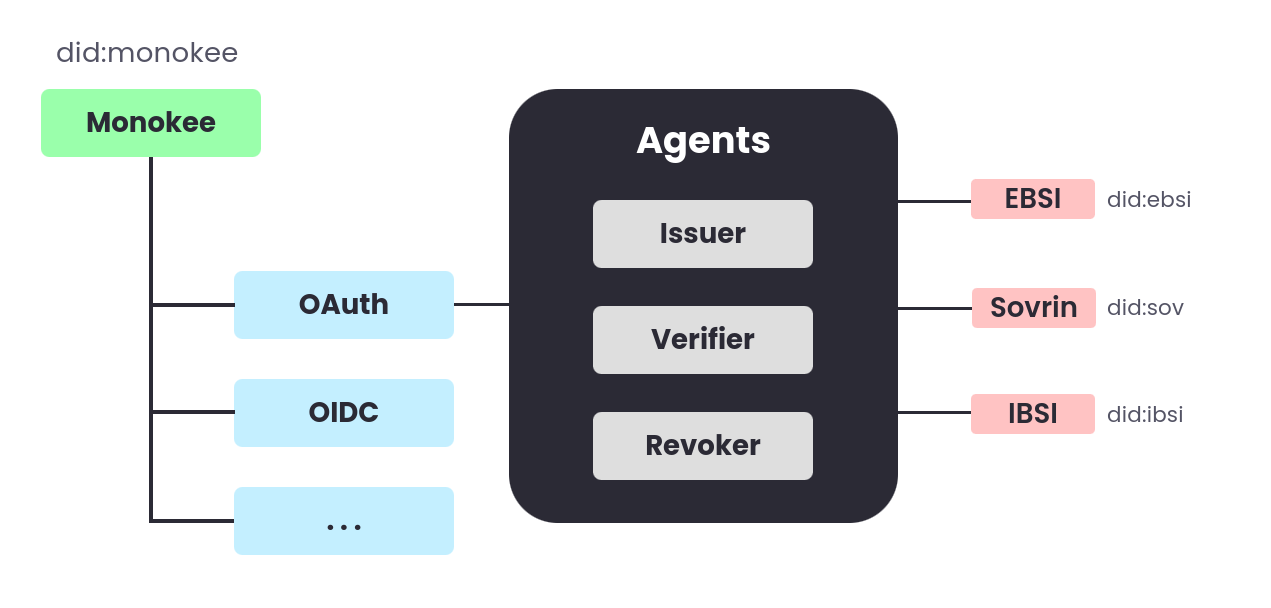
\includegraphics[scale=0.28]{chapter3/problem_schema.png}
    \captionof{figure}{Ideally, Monokee will have its own DID method (did:monokee), 
    through which will be generated identifiers that will hide (at least, as far as 
    the user is concerned) the blockchain where it is located.}
\end{center}
\vspace*{0.5cm}
The final software structure has three main components:
\begin{itemize}
    \item \textbf{Frontend}: it allows the user to interact with the system's core 
    functionalities and serves as an interface for every SSI Kit SDK function.
    \item \textbf{Backend}: it is needed for security, as we will analyze 
    further, and for cryptographic functions that the frontend could not execute.
    \item \textbf{SSI Kit SDK}: it exposes all the SSI functionalities, and enables 
    the user to create keys and DIDs, issue VC, present them as VPs, and more.
    \item \textbf{Smart Contracts}: for what concerns SSI Kit integration, the 
    contracts serve as trusted verifiers and verification results register. Some 
    contracts emit ERC-721 tokens, which let the user request the diploma, but they 
    will not be discussed here.
\end{itemize}
\begin{center}
    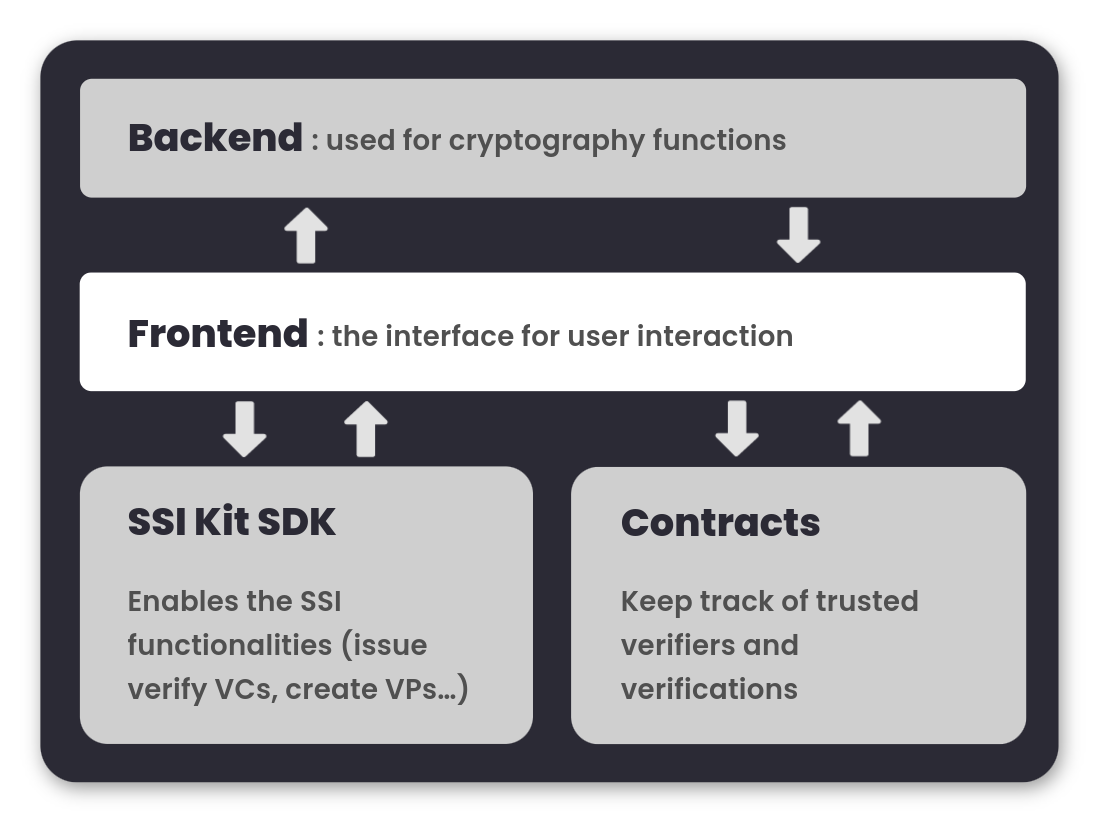
\includegraphics[scale=0.23]{chapter3/structure.png}
    \captionof{figure}{Solution visual representation}
\end{center}

\clearpage
\section{Solution development}
In the following sections, we discuss the technologies we used to build the
solution, and we explain the main functionalities of the system.
\subsection{Technologies and Tools}
Before explaining the solution, we list the languages and tools we leveraged to develop it,
for both SSI Kit SDK and PoC.

\subsubsection{Common tools and languages}
\begin{itemize}
    \setlength\itemsep{-0.1em}
    \item \texttt{Typescript}: a strongly typed programming language that builds 
    on JavaScript. It was chosen because the other Monokee's modules were in 
    Typescript, so it would have been easier for the team to integrate. Also, it is 
    very convenient for its strongly typed nature;
    \item \texttt{JSON}: as already covered in \hyperref[subsubsec:json]{Chapter 2}, 
    JSON is a lightweight data-interchange format. It has been extensively used,
    mainly for credentials representation and API calls;
    \item \texttt{Node.js}: a JavaScript runtime built on Chrome's V8 JavaScript
    engine. It has been used for code execution;
    \item \texttt{npm}: a package manager for the JavaScript programming language.
    It has been used to manage the dependencies of the projects;
    \item \texttt{Git}: a free and open-source distributed version control system
    used for tracking and collaboration purposes;
    \item \texttt{Visual Studio Code}: the Integrated Development Environment (IDE)
    we have used for the solution development.
    
\end{itemize}

\subsubsection[SSI Kit SDK]{SSI Kit SDK\footnote{\texttt{uuid}, \texttt{rfc4648}, \texttt{sha256}, 
and \texttt{nacl} have been used just to generate tokens used for credentials 
revocation, as will be further explained}}

\begin{itemize}
    \setlength\itemsep{-0.1em}
    \item \texttt{jest}: a JavaScript testing framework. It has been used to test
    the SSI Kit SDK components;
    \item \texttt{waltid-ssikit}: the library written in Kotlin/Java that provides 
    the SSI functionalities set. The developed SDK is a Typescript wrapper of this 
    library;
    \item \texttt{axios}: a promise-based HTTP client for the browser and node.js,
    used to make API calls to waltid-ssikit;
    \item \texttt{uuid}: a library used to generate RFC-compliant Universally Unique
    Identifiers (UUIDs);
    \item \texttt{rfc4648}: a library used to encode and decode data in Base32 format;
    \item \texttt{sha256}: a library used to generate SHA-256 hashes;
    \item \texttt{nacl}: a library used to decode UTF8 strings;
\end{itemize}

\subsubsection{Frontend}
\begin{itemize}
    \setlength\itemsep{-0.1em}
    \item \texttt{React.js}: a JavaScript library for building user interfaces. It
    has been used to build the frontend;
    \item \texttt{Chakra-UI}: a simple, modular and accessible components library,
    used with \texttt{React.js} to build the frontend.
    \item \texttt{ethers}: a library used to interact with Ethereum Virtual
    Machine compatible blockchains;
    \item \texttt{wagmi}: a collection of React Hooks containing everything needed
    to start working with Ethereum; it has been used to interact with the smart
    contracts;
    \item \texttt{RainbowKit}: RainbowKit is a React library that makes it easy to 
    add the wallet connection, e.g., for Metamask integration.
    \item \texttt{GraphQL}: the query language used by The Graph;
    \item \texttt{ssikit-sdk}: the developed Typescript SDK used to interact with 
    the SSI Kit library.
    \item \texttt{The Graph}: a decentralized protocol for indexing and querying
    data from blockchains, starting with Ethereum. It makes it possible to query 
    data that is difficult to query directly. It has been used to query The
    deployed smart contracts.
    \item \texttt{smart contracts suite}: a collection of smart contracts used to
    register the verifications and the verification results on-chain.
\end{itemize}

\subsubsection{Backend}
\begin{itemize}
    \setlength\itemsep{-0.1em}
    \item \texttt{Express.js}: a web application framework for Node.js. It has been
    used to build the backend, where the cryptographic functions are executed; the frontend
    calls them through API calls;
    \item \texttt{ssikit-sdk}: the developed Typescript SDK used to interact with
    the SSI Kit library.
    \item \texttt{jose}: a library used to encode and decode JSON Web Tokens (JWTs),
    which have been used to represent private and public keys;
    \item \texttt{nodemon}: a tool that automatically restarts the node application
    when file changes in the directory are detected.
\end{itemize}

\subsection{SSI Kit SDK development}
\subsection{Smart Contract integrations - Web App Proof of Concept}

\section{Discussion}
\subsection{Achievements}
\subsection{Acquired knowledge}
\subsection{Future developments}
\subsection{Personal evaluation}
